\chapter{Ranking}
\textbf{Ranking} is the application of machine learning, typically supervised or reinforcement learning, in the construction of ranking models for information retrieval systems. Training data consists of lists of items with some partial order speicified between items in each list. This order is typically induced by giving a numerical or ordinal score or a binary judgement for each item. 

The ranking model purposes to rank, i.e. producing a permutation of items in new, unseen lists in a similar way to rankings in the training data.

\begin{figure}[h]
    \centering
    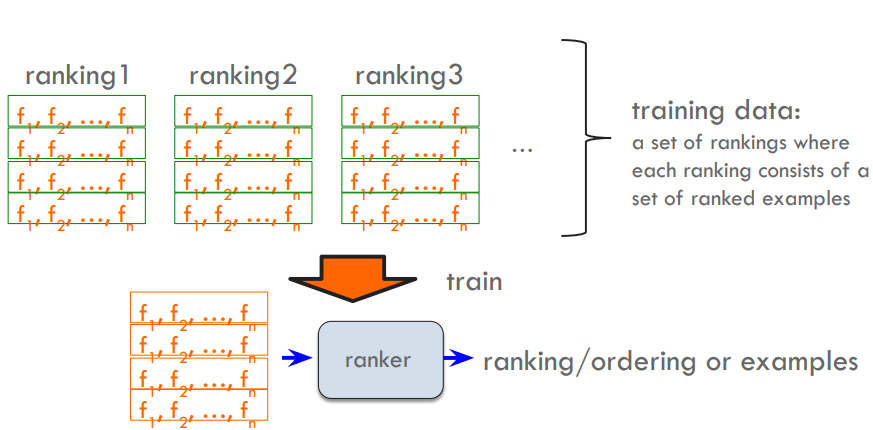
\includegraphics[width=.75\textwidth]{046}
    \caption{Ranking problems general schema.}
\end{figure}

Traditional machine learning solves a prediction problem on a single instance at a time. The aim of traiditional machine learning is to come up with a class or a single numerical score for that instance. Instead, ranking solves a ranking problem on a list of items. The aim of ranking is to come up with optimal ordering of those items. Ranking doesn't care much about the exact score that each item gets, but cares more about the relative ordering among the items.

\section{Multilabel classification}
In machine learning, \textbf{multilabel classification} and the strongly related problem of \textbf{multi-output classification} are varients of the classification problem where multiple labels may be assigned to each instance. Multilabel classification is a generalization of multiclass classification, which is the single-label problem of categorizing instances into precisely one of more than two classes; in the multi-label problem there is no constraint on how many of the classes the instance can be assigned to.

In multiclass classification each example has one label and exactly one label. In multilabel classification each example has \textbf{zero or more labels}.

Formally, multilabel classification is the problem of finding a model that maps inputs \(\vec{x}\) to binary vectors \(\vec{y}\) (assigning a value of 0 or 1 for each element - label - in \(\vec{y}\)).

Multilabel applications examples are:
\begin{itemize}[topsep={0pt}, partopsep={0pt}]
    \item Video surveillance - reidentification;
    \item Scene analysis - visual localization;
    \item Image annotation;
    \item Document topics;
    \item Medical diagnosis.
\end{itemize}

\section{Ranking problems}
Suppose we start a new web search company. Like other search engines, a userinputs a query and a set of documents is retrieved. Our goal is to rank the resulting documents based on relevance to the query. The ranking problem is to take a collection of items and sort them according to some notion of preference. One of the trickiest parts of doing ranking through learning is to properly define the loss function.

\subsection{Black box approach}
We can implement the algorithm for the preference function with the perceptron by creating the vector of the features of the two examples.

Given a generic binary classifier, we can use it to solve our new problem.
\begin{figure}[t!]
    \centering
    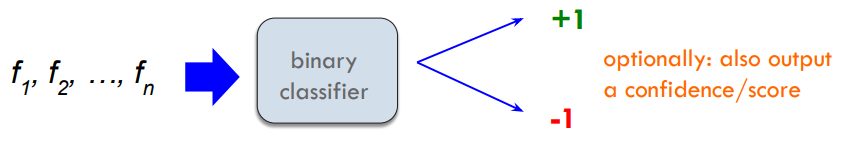
\includegraphics[width=1\textwidth]{047}
    \caption{Black box approach to ranking.}
\end{figure}
We need to train a classifier to decide if the first input is better than the second: we have to consider all the possible pairings of the examples in a ranking and label them as positive if the first example is higher ranked, otherwise we rank them as negative.

The problem here is that our binary classifier takes only one example as input. How can we perform the following classification?
\begin{equation}
    a_1, a_2, ..., a_n; b_1, b_2, ..., b_n \to f_1', f_2', ... f_n'
\end{equation}
We need features that compare the two examples \(a_i\) and \(b_i\), this new vector is called \textbf{combined feature vector}. There are many approaches that depend on domain and on the classifier, two common approaches to do this are:
\begin{itemize}
    \item compare by difference:
    \begin{equation*}
        f'_i = a_i - b_i
    \end{equation*}
    \item compare the first to the second example:
    \begin{equation*}
        f'_i = \begin{cases}
            1 &\text{ if } a_i > b_i\\
            0 &\text{ otherwise}\\
        \end{cases}
    \end{equation*}
\end{itemize}

\subsection{Preference function}
For each query, we are also given a collection of documents, together with a desired ranking over those documents. We'll assume that we have \(N\)-many queries and for each query we have \(M\)-many documents. The goal is to train a binary classifier to predict a \textbf{preference function}. Given a query \(q\) and two documents \(d_i\) and \(d_j\), the classifier should predict whether \(d_i\) should be preferred to \(d_j\) with respect to the query \(q\).

\subsection{Bipartite Ranking}
Bipartite ranking algorithms are useful for bipartite ranking problems. A \textbf{Bipartite ranking problem} is one in which you are trying to predict a binary response, for instance "is this document relevant or not?".

The only goal is to ensure that all the relevant documents are ahead of all the irrelevant documents. There is no notion that one relevant document is more relevan than another.

For non-bipartite ranking problems, more sophisticated methods can be used.

\begin{figure}[t!]
    \centering
    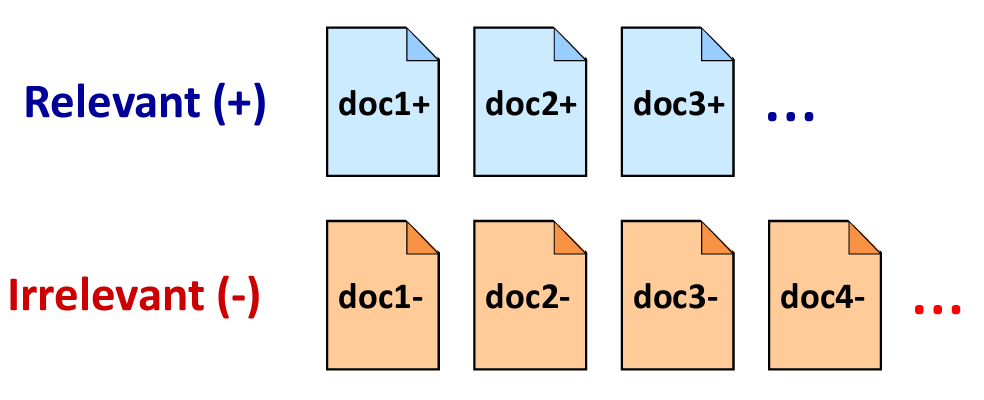
\includegraphics[width=0.75\textwidth]{099}
    \caption{Bipartite ranking example}
\end{figure}

\section{Algorithm}
A naive solution for the training algorithm of the ranking is pretty simple. As we sayed, the goal is to predict a preference function that, given a query and two documents, the clasifier should predict whether the first should be preferred to the second with respect to the query. In the following algorithm, we will assume \(N\)-many queries and for each quary we have \(M\)-many documents. 

For every \(n\) and every pair \(i \neq j\), we wil create a binary classification example based on features \(\vec{x}_{nij}\) (that denotes the features associated with comparing document \(i\) to document \(j\) on query \(n\)). This example is positive if \(i\) is preferred to \(j\), otherwise it is negative.

\begin{algorithm}
    \caption{NaiveRankTrain(RankingData, BinaryTrain)}
    \label{alg:naive_rank_train}
$D \gets [\ ]$\;
\For{$n \gets 1$ to $N$}{
    \For{$i,j \gets 1$ to $M$ and $i \neq j$}{
     \eIf{$i$ is preferred to $j$ on query $n$}{
            $D \gets D.append(\vec{x}_{nij},+1)$\;
        }{
            \If{$j$ is preferred to $i$ on query $n$}{
                $D \gets D.append(\vec{x}_{nij},-1)$\;
            }
        }
    }
}
\Return{BinaryTrain($D$)}
\end{algorithm}

We can describe a naive solution for the test phase as well. In this case we initialize a list of scorest to 0, than for each document \(d_i\) and \(d_i\) (\(i \neq j\)), we compute the score with our preference function; then we add the score to \(d_i\) and subtract the score to \(d_j\). At the end we return the queries sorted by the computed scores.

\begin{algorithm}
    \caption{NaiveRankTest($f$, $\hat{x}$)}
    \label{alg:naive_rank_test}
$score \gets \langle 0, 0, ..., 0 \rangle$\;
\For{$i,j \gets 1$ to $M$ and $i \neq j$}{
    $y \gets f(\hat{x}_{ij})$\;
    $score_i \gets score_i + y$\;
    $score_j \gets score_j - y$\;
}
\Return{$score$.sort()}
\end{algorithm}

The problem with this approach is that it's impossible to tell --- just by looking at its output on one \(i,j\) pair --- how good the overall ranking is. This is because there is the intermediate step of turning these pariwise predictions into a coherent ranking.

These algorithms actually work quite well in the case of bipartite ranking problems. This is essentially beause the only goal in bipartite ranking problems is to ensure that all the relevant documents are ahead of all the irrelevant documents. 

\section{Weighted binary classification}
For non-bipartite ranking problems, we can do better. First, when the preferences thath we get at training time are more nuanced than "relevant or not", we can incorporate these preferences at training time. Effectively, we want to give a higher weight to binary problems that are very different in terms of preference than others. Second, rather than producing a list of scores and then calling an arbitrary sorting algorithm, we can actually use the preference function as the sorting function inside our own implementation of quicksort.

Define a ranking as a function \(\sigma\) that maps the objects we are ranking to the desired position in the list \(1,2,...,M\). If \(\sigma_u < \sigma_v\) then \(u\) is preferred to \(v\). Given data with observed rankings \(\sigma\), our goal is to learn to predict rankings for new objects, \(\hat{\sigma}\). We define \(\Sigma_M\) as the set of all ranking functions over \(M\) objects. We also wish to express the fact that making a mistake on some pairs is worse than making a mistake on others - this will be encoded in a cost function \(\omega\), where \(\omega(i,j)\) is the cost for accidentally putting something in position \(j\) when it should have gone in position \(i\). To be a valid cost function, \(\omega\) should be \emph{symmetric}, \emph{monotonic}: if \(i < j < k\) then \(\omega(i,j) \leq \omega(i,k)\), \emph{satisfy the triangle inequality}: \(\omega(i,j) + \omega(j,k) \geq \omega(i,k)\).

\subsection{\(\omega\)-Ranking}
Given an input space \(\mathcal{X}\), an unknown distribution \(\mathcal{D}\) over \(\mathcal{X} \times \Sigma_M\), and a training set \(D\) sampled from \(\mathcal{D}\).\\
We want to compute a function \(f : \mathcal{X} \to \Sigma_M\) minimizing:
\begin{equation}
    \mathbb{E}_{(\vec{x},\sigma) \sim \mathcal{D}} \left[ \sum_{u \neq v} [\sigma_u < \sigma_v][\hat{\sigma}_v < \hat{\sigma}_u] \omega ( \sigma_u , \sigma_v ) \right]
\end{equation}
where \(\hat{\sigma} = f(\vec{x})\).

In this definition, the only complex aspect is the loss function. This loss sums over all pairs of objects \(u\) and \(v\), but the predicted ranking \(\hat{\sigma}\) prefers \(v\) to \(u\), then you incur a cost of \(\omega(\sigma_u,\sigma_v)\).

Depending on the problem you care about, you can set \(\omega\) to many "standard" options. If \(\omega(i,j) = 1\) whenever \(i \neq j\), then you achieve the Kemeny distance measure, which simly counts the number of airwise misordered items. We may only care about getting the top \(K\) predictions correct. In this case, we define:
\begin{equation}
    \omega(i,j) = \begin{cases}
        1 &\text{if min}\{i,j\} \leq K \text{ and } i \neq j\\
        0 &\text{otherwise}\\
    \end{cases}
\end{equation}
In this case, only errors in the top \(K\) elements are penalized. Swapping items 55 and 56 is irrelevent (for \(K < 55\)).

\begin{algorithm}
    \caption{RankTrain($D^\text{rank}$, $\omega$, BinaryTrain)}
    \label{alg:rank_train}
$D^\text{bin} \gets [\ ]$\;
\For{$(\vec{x},\sigma) \in D^\text{rank}$}{
    \For{$u \neq v$}{
        $y \gets \text{sign}(\sigma_v - \sigma_u))$\;
        $w \gets \omega(\sigma_u - \sigma_v)$\;
        $D^\text{bin} \gets D^\text{bin} \oplus (y,w,\vec{x}_{uv})$\;
    }
}
\Return{BinaryTrain($D^\text{bin}$)}
\end{algorithm}

At test time, instead of predicting scores and then sorting hte list, as in the previous algorithm, we run the quicksort algorithm, using the learned function as a comparison function. In practice at teach step a pivot \(p\) is chosen. Every object \(u\) is compared to \(p\) using the learned function and sorted to left or right. The difference between this algorithm and quicksort is that the comparison function is \emph{probabilistic}. If \(f\) outputs probabilities, for instance it predicts that \(u\) has an 80\% probability of being better than \(p\), then it puts it on the left with 80\% probability and on the right with 20\% probability.

\begin{algorithm}
    \caption{RankTest($f$, $\hat{x}$, $obj$)}
    \label{alg:rank_test}
\eIf{$obj$ contains 0 or 1 elements}{
    \Return{$obj$}
}{
    $p \gets$ randomly chosen object in $obj$\;
    $left \gets [\ ]$\;
    $right \gets [\ ]$\;
    \For{$u \in obj \setminus \{p\}$}{
        $\hat{y} \gets f(\vec{x}_{up})$\;
        \eIf{uniform random variable < $\hat{y}$}{
            $left \gets left \oplus u$\;
        }{
            $right \gets right \oplus u$\;
        }
    }
    $left \gets $ RankTest($f, \hat{x}, left$)\;
    $right \gets $ RankTest($f, \hat{x}, right$)\;
}
\Return{$left \oplus \langle p \rangle \oplus right$}
\end{algorithm}
This algorithm is better than the naive algorithm in at least two ways. First, it only makes \(O(M \log_2 M)\) calls to \(f\) rather than \(O(M^2)\) calls in the naive case. Second, it achieves a better error bound.

\newpage\null
\newpage
\begin{exercise}[topsep=20pt,itemsep=10pt]
    \ex[!] Describe the ranking.
    \ex What is multilabel classification? Give some application example.
    \ex[!] Can I use the perceptron to do ranking?
    \ex What is the preference function?
    \ex Describe the bipartite ranking problem.
    \ex[!] How can the binary classifier problem be solved?
    \ex Describe the weighted binary classification.
    \ex Provide and describe the weighted ranking training algorithm.
    \ex Provide and describe the weighted ranking testing algorithm.
\end{exercise}
